%%%%%%%%%%%%%%%%%%%%%%%%%%%%%%%%%%%%%
%                                   %
% Compile with XeLaTeX and biber    %
%                                   %
% Questions or comments:            %
%                                   %
% joshua dot mcneill at uga dot edu %
%                                   %
%%%%%%%%%%%%%%%%%%%%%%%%%%%%%%%%%%%%%

\documentclass{beamer}
  % Read in standard preamble (cosmetic stuff)
  %%%%%%%%%%%%%%%%%%%%%%%%%%%%%%%%%%%%%%%%%%%%%%%%%%%%%%%%%%%%%%%%
% This is a standard preamble used in for all slide documents. %
% It basically contains cosmetic settings.                     %
%                                                              %
% Joshua McNeill                                               %
% joshua dot mcneill at uga dot edu                            %
%%%%%%%%%%%%%%%%%%%%%%%%%%%%%%%%%%%%%%%%%%%%%%%%%%%%%%%%%%%%%%%%

% Beamer settings
% \usetheme{Berkeley}
\usetheme{CambridgeUS}
% \usecolortheme{dove}
% \usecolortheme{rose}
\usecolortheme{seagull}
\usefonttheme{professionalfonts}
\usefonttheme{serif}
\setbeamertemplate{bibliography item}{}

% Packages and settings
\usepackage{fontspec}
  \setmainfont{Charis SIL}
\usepackage{hyperref}
  \hypersetup{colorlinks=true,
              allcolors=blue}
\usepackage{graphicx}
  \graphicspath{{../../figures/}}
\usepackage[normalem]{ulem}
\usepackage{enumerate}

% Document information
\author{M. McNeill}
\title[FREN2001]{Français 2001}
\institute{\url{joshua.mcneill@uga.edu}}
\date{}

%% Custom commands
% Lexical items
\newcommand{\lexi}[1]{\textit{#1}}
% Gloss
\newcommand{\gloss}[1]{`#1'}
\newcommand{\tinygloss}[1]{{\tiny`#1'}}
% Orthographic representations
\newcommand{\orth}[1]{$\langle$#1$\rangle$}
% Utterances (pragmatics)
\newcommand{\uttr}[1]{`#1'}
% Sentences (pragmatics)
\newcommand{\sent}[1]{\textit{#1}}
% Base dir for definitions
\newcommand{\defs}{../definitions}


  % Packages and settings

  % Document information
  \subtitle[Nécessité]{Les expressions de nécessité}

\begin{document}
  % Read in the standard intro slides (title page and table of contents)
  \begin{frame}
    \titlepage
    \tiny{Office: % Basically a variable for office hours location
Gilbert 121\\
          Office hours: % Basically a variable for office hours
 lundi, mercredi, vendredi 10:10--11:10
}
  \end{frame}

  \begin{frame}{Annonces}
    \begin{itemize}
      \item Le devoir 4 est disponble sur eLC et à rendre le 27 mars.
      \item[] \tinygloss{Homework 4 is available on eLC and due March 27th.}
    \end{itemize}
  \end{frame}

  \begin{frame}{S'habiller pour l'occasion}
    \begin{columns}
      \column{0.5\textwidth}
        Quand est-ce qu'\alert{il faut mettre} ces vêtements?
        Pensez à une activité ou au temps.
        \begin{enumerate}
          \item un anorak
          \item<2-> des sandales
          \item<3-> un imperméable
          \item<4-> des lunettes de soleil
          \item<5-> des gants
        \end{enumerate}
      \column{0.5\textwidth}
        \begin{minipage}[c][0.8\textheight]{\linewidth}
          \begin{center}
            \only<1>{
              
\includegraphics[scale=0.15]{kenny.jpg}
            }
            \only<2>{
              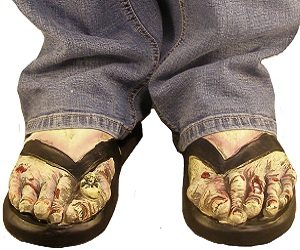
\includegraphics[scale=0.5]{sandales.jpg}
            }
            \only<3>{
              \includegraphics[scale=0.2]{imperméable.jpg}
            }
            \only<4>{
              
\includegraphics[scale=0.3]{lunettes.jpg}
            }
            \only<5>{
              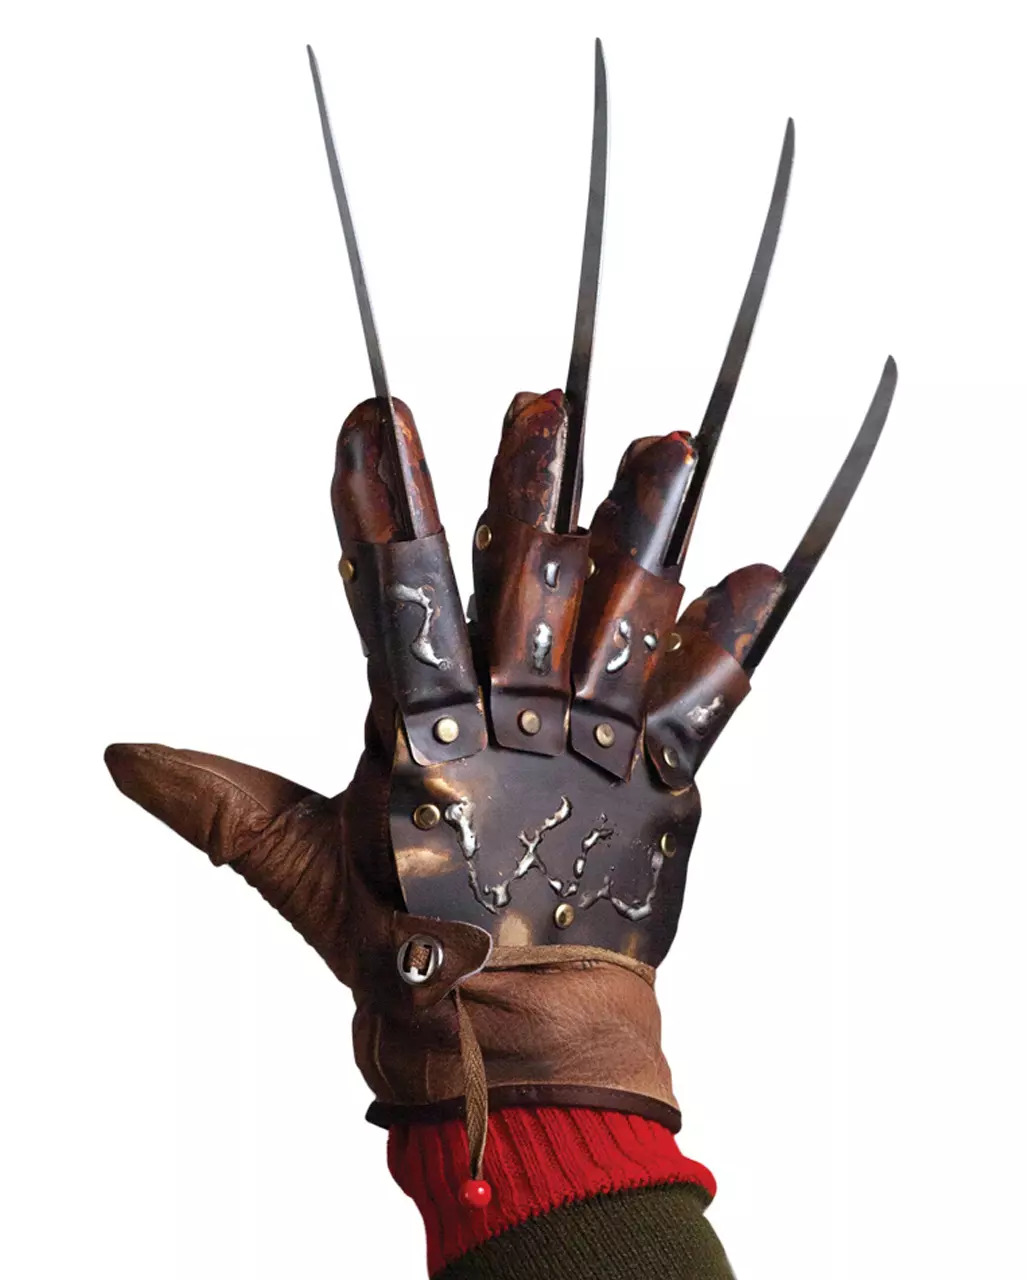
\includegraphics[scale=0.15]{gants.jpg}
            }
          \end{center}
        \end{minipage}
    \end{columns}
  \end{frame}

  \begin{frame}{}
    \begin{center}
      \Large Quiz
    \end{center}
  \end{frame}

  \begin{frame}{Des conseils}
    \small
    En groupes de 3 ou 4, donnez des conseils pour bien réussir les situations indiquées.
    \begin{description}
      \item[] \textbf{Modèle:} \emph{pour passer les grandes vacances avec des amis}
      \item[E1:] \emph{Il faut} louer ...
      \item[E2:] \emph{Il est utile d}'organiser ...
      \item[E3:] \emph{Il est important de} sortir ...
    \end{description}
    \begin{columns}[t]
      \column{0.5\textwidth}
        \begin{enumerate}
          \item pour organiser une fête d'anniversaire pour un/e ami/e
          \item pour planifier un grand repas de famille
          \item pour assister à un mariage
        \end{enumerate}
      \column{0.5\textwidth}
        \begin{enumerate}
          \setcounter{enumi}{3}
          \item pour passer les grandes vacances en famille
          \item pour fêter Thanksgiving avec la famille
          \item pour célébrer Halloween avec des amis
        \end{enumerate}
    \end{columns}
  \end{frame}

  \begin{frame}{}
    \begin{center}
      \Large Questions?
    \end{center}
  \end{frame}
\end{document}
